% Closing slide: thank you, over a screenshot of the team's video call.
% Written by Claude Opus 5.5 (Claude Code), 2026-11-15. Photo: video_call.jpg (supplied by Syoma).
\documentclass[aspectratio=169]{beamer}
\usepackage{tikz}
\usepackage{mathpazo}
\usepackage[scaled=0.92]{helvet}
\setbeamertemplate{navigation symbols}{}
\definecolor{accent}{RGB}{214,110,80}
\definecolor{cream}{RGB}{240,237,229}
\definecolor{callbg}{RGB}{12,16,19}
\setbeamercolor{background canvas}{bg=callbg}
\begin{document}
\begin{frame}[plain]
\begin{tikzpicture}[remember picture,overlay]
  \node[inner sep=0,anchor=center] at (current page.center)
    {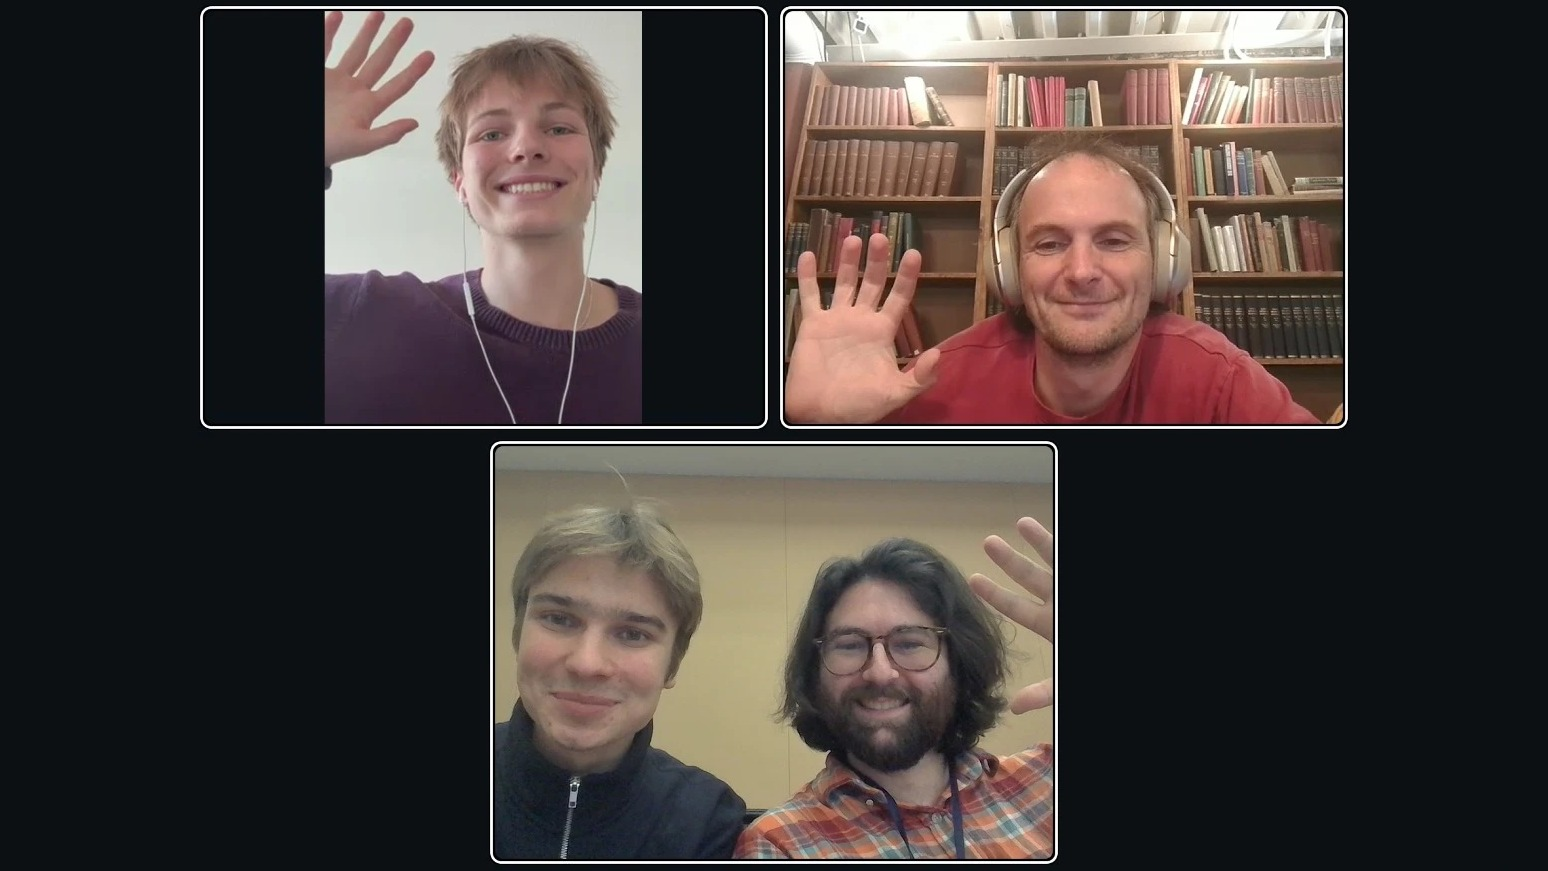
\includegraphics[width=\paperwidth,height=\paperheight]{video_call.jpg}};
  % bottom left, in the dark area beside the lower video tile
  \node[anchor=south west,inner sep=0,align=left,text width=4.2cm]
    at ([xshift=0.55cm,yshift=1.5cm]current page.south west) {%
    {\fontfamily{phv}\selectfont\scriptsize\bfseries\color{accent} PROBLEM 137\par}\vspace{3pt}
    {\fontfamily{ppl}\selectfont\fontsize{30}{32}\selectfont\bfseries\color{cream} Thank\ you!\par}};
  % bottom right
  \node[anchor=south east,inner sep=0,align=right,text width=4.2cm]
    at ([xshift=-0.55cm,yshift=1.5cm]current page.south east) {%
    {\fontfamily{phv}\selectfont\normalsize\bfseries\color{cream} Mighty Math Magicians\par}\vspace{3pt}
    {\fontfamily{phv}\selectfont\scriptsize\color{cream!70} Caltech Mathathon 2026\par}\vspace{8pt}
    {\fontfamily{ppl}\selectfont\large\bfseries\color{accent} Questions?\par}};
\end{tikzpicture}
\end{frame}
\end{document}
